\section{Results}
\label{sec:results}

We test the four proposed dispatching strategies in the Zurich scenario with four runs per strategy. Each run simulates 20 iterations to allow the dispatchers to sense the traffic conditions in the network, i.e. to figure out what travel times on specific links are expected and how traffic jams can be avoided.

[TODO : From here the plots are new! Rework interpretation! also, 10 runs each are running at the moment]

Figure \ref{fig:mean_peak_waiting_times} shows the waiting times for customers at peak hours. In order to arrive at that measure the 24 five minute time bins with the highest average waiting time have been selected. Then, all the waiting times that occured within selected bins are averaged. One can see that the load-balancing heuristic is performing worse almost over the whole range of fleet sizes, while the two rebalancing algorithms provide the shortest wait times. The bipartite matching approach lies in between. This makes sense, since both LPs are based on the bipartite matching with additional rebalancing added.

Only for very small fleet sizes the rebalancing approaches perform worse. This can be explained by the shifting of daily travel plans. If the peoples' trips in the morning take too long they may be delayed extremely in their daily plans and therefore the travel demand that is assumed for the LP at different times of the day does not match the actual emerging trip distribution.

\begin{figure}
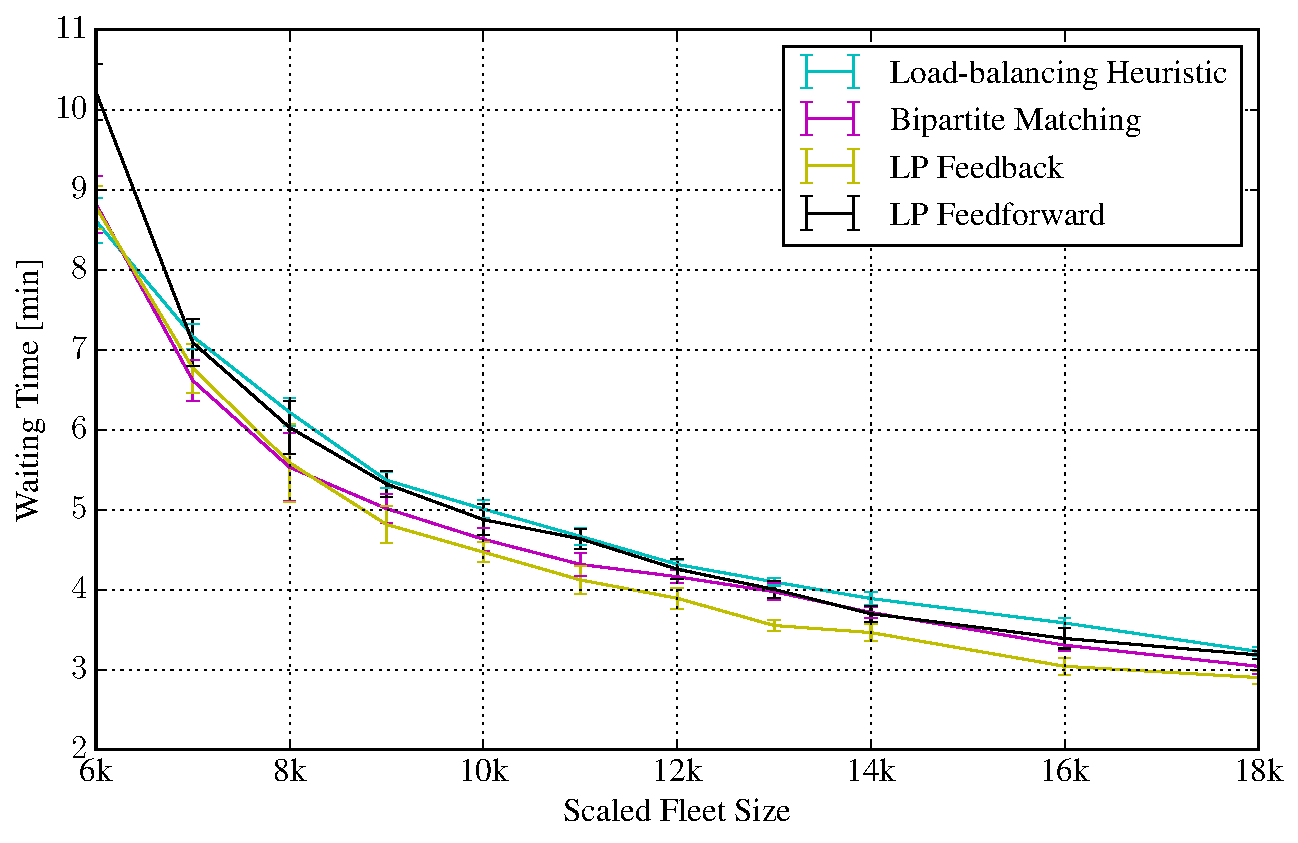
\includegraphics[width=1.0\textwidth]{figures/mean_peak_waiting_times.pdf}
\label{fig:mean_peak_waiting_times}
\caption{Mean peak waiting times}
\end{figure}

\begin{figure}
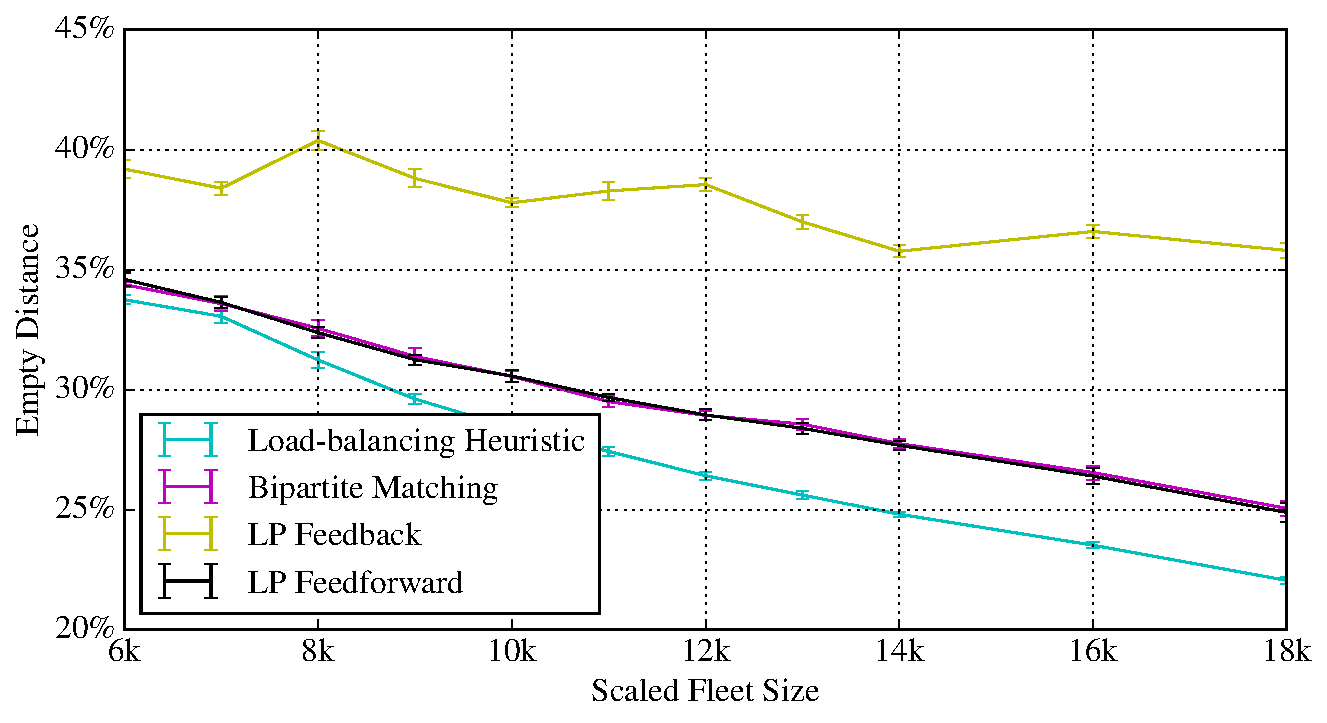
\includegraphics[width=1.0\textwidth]{figures/empty_rides.pdf}
\label{fig:empty_rides}
\caption{Empty Rides}
\end{figure}

On the flipside, the miles driven without a passenger are much lower for the heuristic as can be seen in Figure \ref{fig:empty_rides}. While for the feedback dispatcher half of the miles driven are used for pickup trips and rebalancing, an increased fleet size has a large impact on the distance efficiency of the fleet for the heuristic. The feed-foward LP performs better than the feedback version since the information on when and where trips will take place is better than for the former one. Finally, the bipartite matching algorithm performs better than the LPs but worse than the simple heuristic. This is due to pickup trips that may be diverted. [TODO: And? Actually the sole purpose is to minimize distance, isn't it?]

\begin{figure}
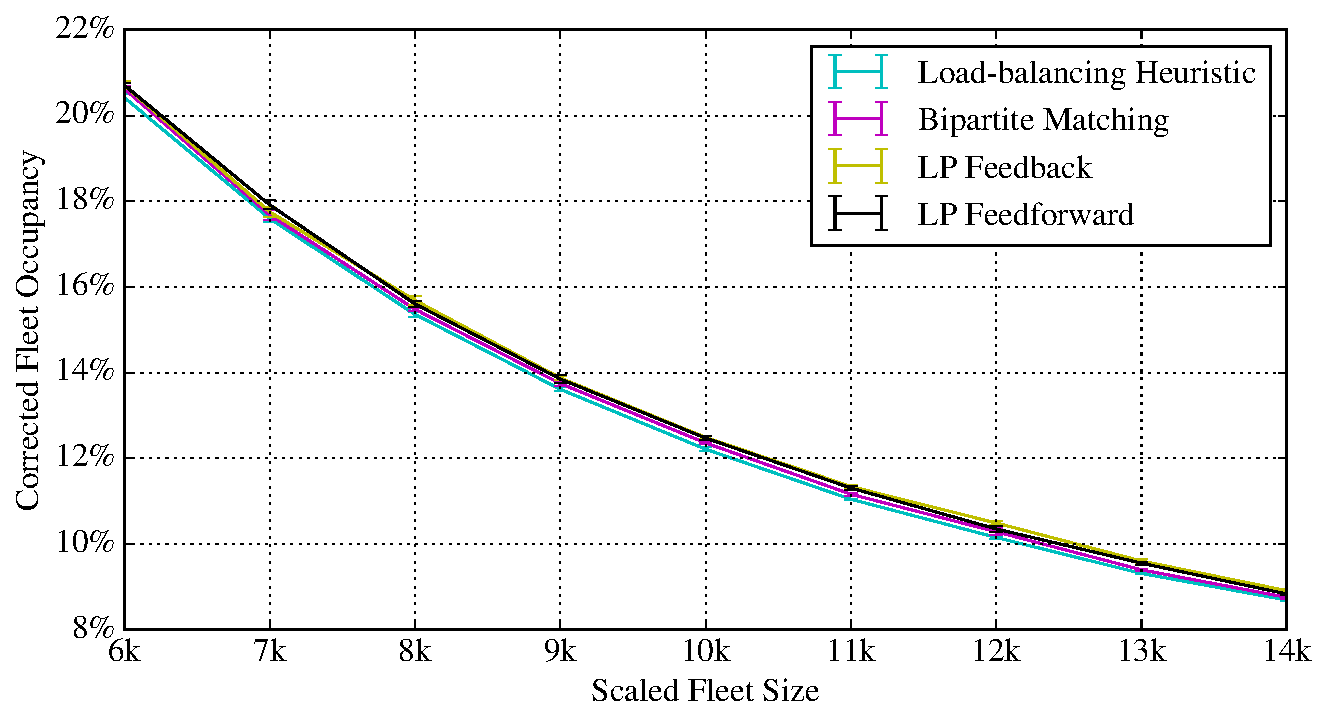
\includegraphics[width=1.0\textwidth]{figures/occupancy.pdf}
\label{fig:occupancy}
\caption{Corrected Fleet Occupancy (factor 24/30) TODO: add today's vehicle fleet occupancy}
\end{figure}

Finally, the fleet occupancy is displayed in Figure \ref{fig:occupancy}. The utilization of the fleet is mainly dependent on fleet size, while the choice of the dispatching strategy is only leading to marginal differences. However, one can see that the utilization of the fleet for the heuristic is constantly lower than for the other dispatchers.

\section{Cost Analysis}
\label{sec:cost_analysis}

The simulation output has been prepared to be compatible with the cost calculator by [cite]. Figure \ref{fig:passenger_price} shows the price per passenger of operating a certain fleet with a specific dispatching algorithm with a profit margin of 3\% (as defined by the cost calculator). While the pricing structure is quite constrained for any strategy for very small fleet sizes, the advanced algorithms outperform the simple heuristic for larger fleets. For instance, for a fleet size of 140000 vehicles, the operator would be able to offer a price of 6 Rp/km less than with the simple heuristic.

\begin{figure}
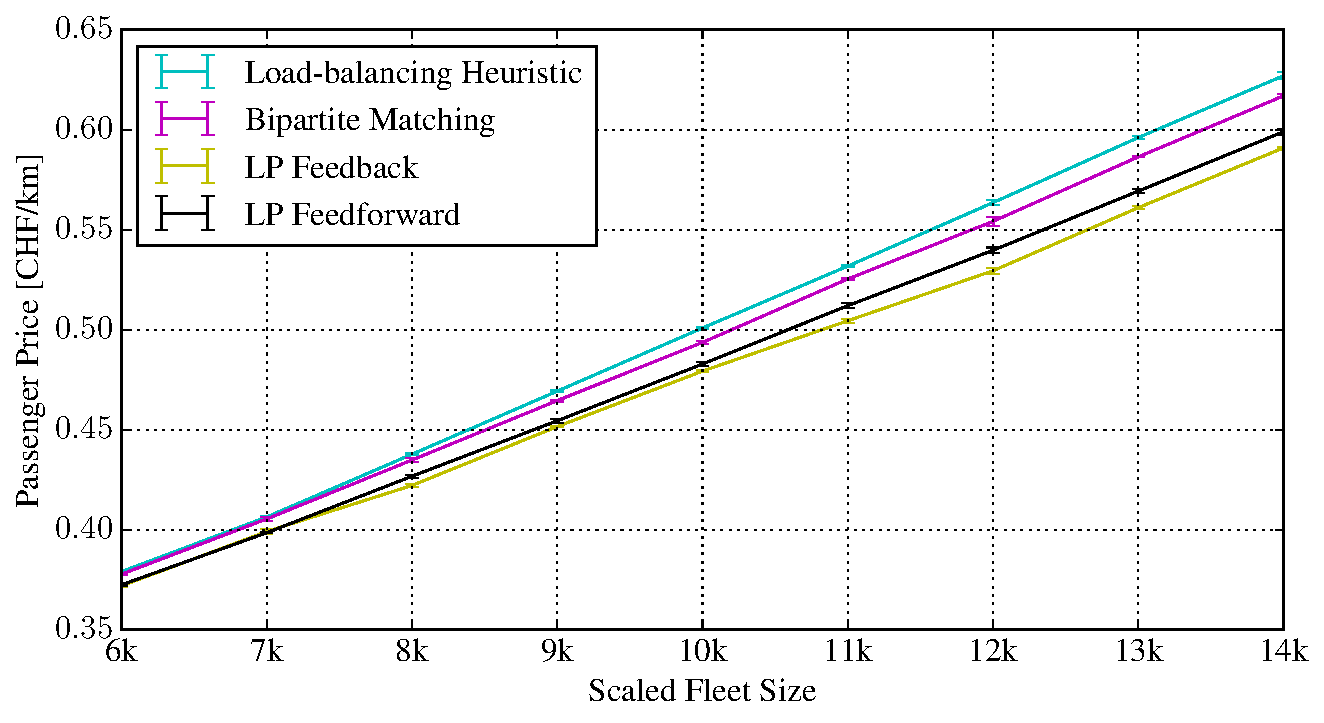
\includegraphics[width=1.0\textwidth]{figures/01_passenger_price.pdf}
\label{fig:passenger_price}
\caption{Price per Passenger Km}
\end{figure}

\begin{figure}
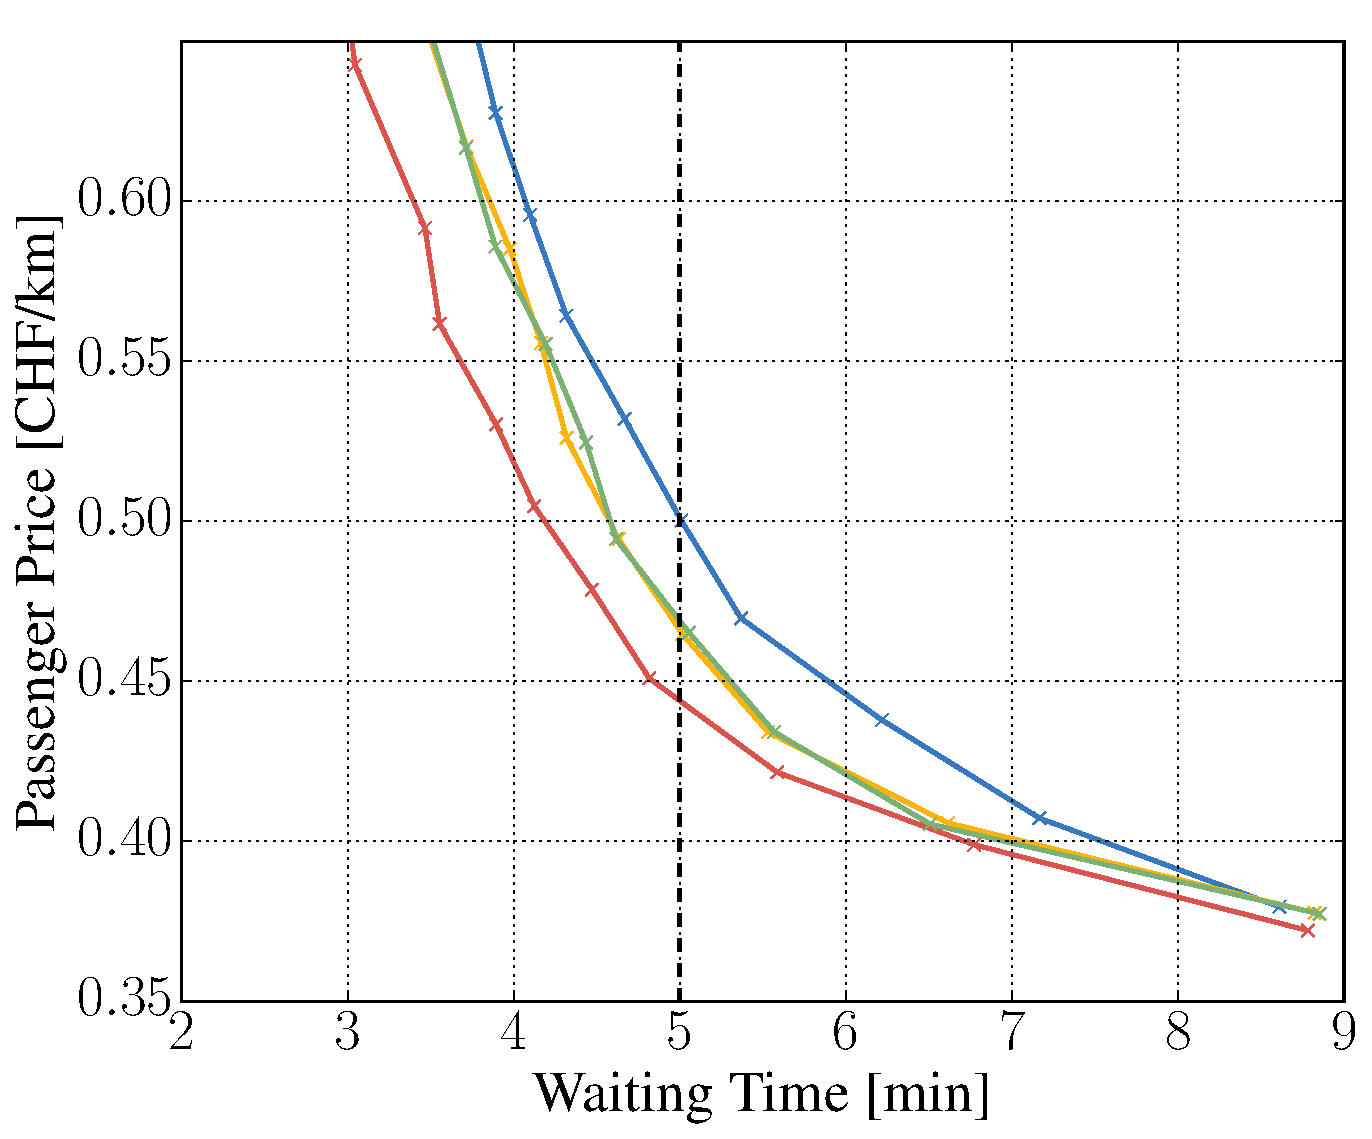
\includegraphics[width=1.0\textwidth]{figures/time_vs_price.pdf}
\label{fig:time_vs_price}
\caption{Time vs. Price}
\end{figure}
